\documentclass[a4paper, 11pt, twocolumn]{article}

\usepackage[a4paper, total={6.24in, 8.5in}]{geometry}
\usepackage[utf8]{inputenc}
\usepackage{graphicx}
\usepackage{verbatim}
\usepackage{float}
\usepackage{array}
\usepackage{xfrac}
\usepackage{mathpazo}
\usepackage{amsmath}
\usepackage{bm}
\usepackage{multirow}
\usepackage{makecell}
\usepackage{multicol}
\usepackage{sectsty,textcase}
\usepackage{wrapfig,lipsum,booktabs}
\usepackage{enumitem}
\usepackage{hyperref}
\usepackage{makecell}
\usepackage{array}
\usepackage{layouts}

\bibliographystyle{plain}
\renewcommand{\thesection}{\arabic{section}}
\setlength{\columnsep}{15pt}
\newcommand{\myparagraph}[1]{\paragraph{#1}\mbox{}\\}

\title{FYS-STK3155/4155 Applied Data Analysis and Machine Learning - Project 3 }

\author{Lotsberg, Bernhard Nornes \\ Nguyen, Anh-Nguyet Lise \and
\url{https://github.com/liseanh/FYS-STK4155-project3}}
\date{November - December 2019}
\begin{document}
\twocolumn[
  \begin{@twocolumnfalse}
    \maketitle
      \begin{abstract}
      We implement and compare k Nearest Neighbours (kNN), a Multilayer Perceptron
      (MLP) and eXtreme Gradient Boosting (XGB) on simulated binary classification 
      data. MLP and XGB perform Similarly when evaluating the test F$_1$ scores, 
      with F$_1\approx 0.87$ and F$_1\approx 0.88$ respectively. kNN performed 
      well despite being a much simpler model, achieving F$_1 \approx 0.83$. 
      Because of the importance of avoiding false negatives and the smaller 
      computational cost of XGB compared to the MLP, we find XGB to be the best 
      method overall for this split of the data. In the future one should look 
      into model stability over several train test splits of the data.
      \end{abstract}
  \end{@twocolumnfalse}
]


\section{Introduction}
A wide array of machine learning methods have been developed over the years for 
various predictive purposes, with the the neural network being the probably most 
well-known method among the general population. In recent years many other 
statistical learning methods have proven themselves as well however. In this 
project we compare the performance of neural networks and gradient boosting in 
the case of binary classification. In addition to these, we also use the much 
simpler k-nearest neighbours method as a baseline for classification performance.



\section{Data}

The data set we will analyse in this project is the MAGIC Gamma Telescope data
set retrieved from the \href{https://archive.ics.uci.edu/ml/datasets/MAGIC+Gamma
+Telescope}{UCI Machine Learning Repository}, which was generated by a Monte
Carlo (MC) program described by D. Heck et. al. \cite{heck1998corsika} to
simulate high energy gamma particle registration in a Cherenkov gamma telescope.
The set consists of ten explanatory variables and a binary response variable
\texttt{class} which specifies whether the measured photons resulted from a gamma
particle (\texttt{class} = g) or a hadron (\texttt{class} = h). The entire data
set consists of 19020 instances with no missing values, with outcome distribution
as shown in Figure \ref{fig:Histogram}. The explanatory and response variables
are defined as the following by the UCI Machine Learning Repository
\cite{Dua:2019}:

\begin{enumerate}[leftmargin=5mm, itemsep=0pt,  parsep=1pt]
  \item \texttt{fLength}: continuous \# major axis of ellipse [mm]
  \item \texttt{fWidth}: continuous \# minor axis of ellipse [mm]
  \item \texttt{fSize}: continuous \# 10-log of sum of content of all pixels
        [in \#phot]
  \item \texttt{fConc}: continuous \# ratio of sum of two highest pixels over
        \texttt{fSize} [ratio]
  \item \texttt{fConc1}: continuous \# ratio of highest pixel over \texttt{fSize}
        [ratio]
  \item \texttt{fAsym}: continuous \# distance from highest pixel to center,
        projected onto major axis [mm]
  \item \texttt{fM3Long}: continuous \# 3rd root of third moment along major
        axis [mm]
  \item \texttt{fM3Trans}: continuous \# 3rd root of third moment along minor
        axis [mm]
  \item \texttt{fAlpha}: continuous \# angle of major axis with vector to origin
        [deg]
  \item \texttt{fDist}: continuous \# distance from origin to center of ellipse
        [mm]
  \item \texttt{class}: g, h \# gamma (signal), hadron (background)
\end{enumerate}

\begin{figure}
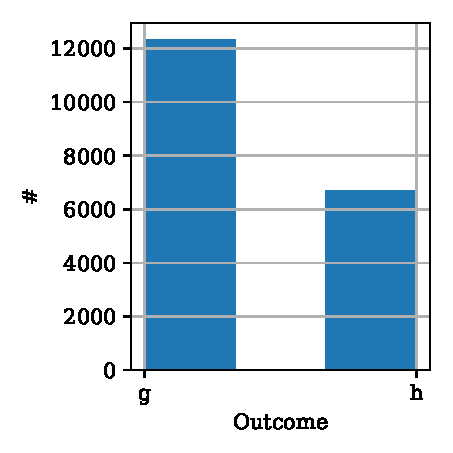
\includegraphics[scale=1]{{figures/histogram}.pdf}
\caption{Frequencies of the outcomes g and h in the data set. The numbers of
instances for the categories were 12332 and 6688 for g and h respectively.}
\label{fig:Histogram}
\end{figure}
The correlation between the features can be seen in Figure \ref{fig:Correlation}.


\begin{figure*}
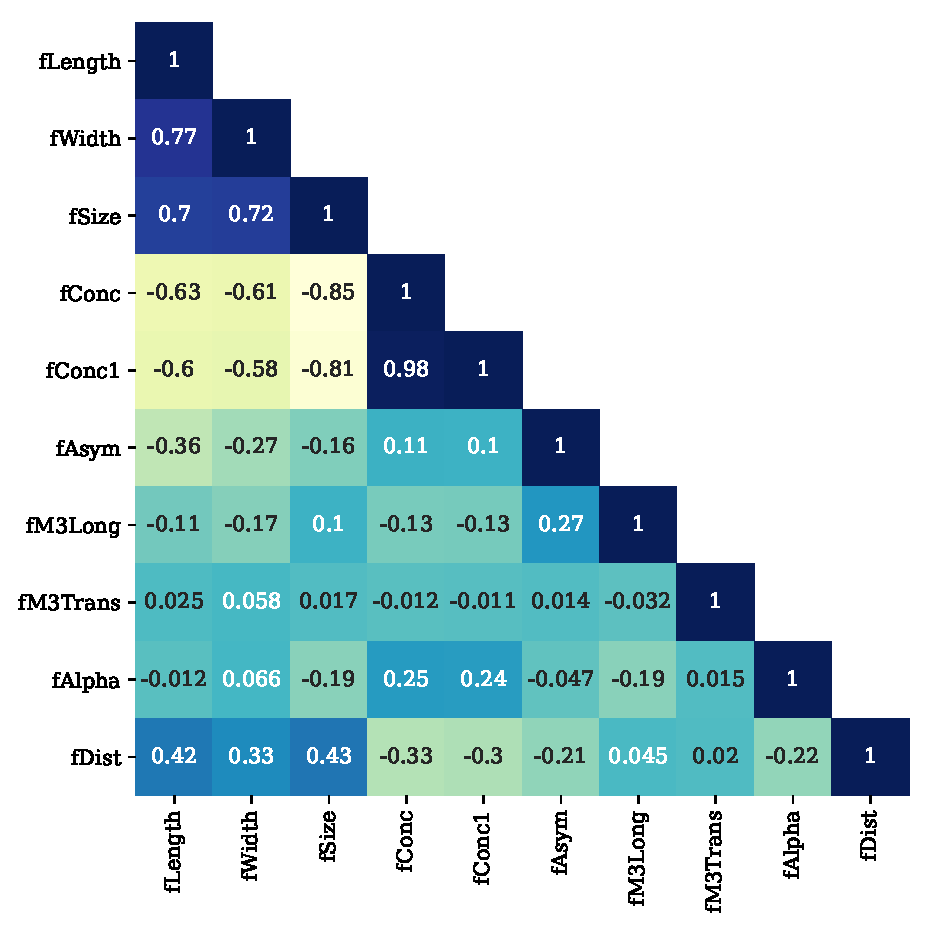
\includegraphics[scale=1]{{figures/correlation_matrix_train}.pdf}
\caption{Correlation matrix of the features in the train set. Upper triangle
excluded for readability.}
\label{fig:Correlation}
\end{figure*}


\subsection*{Preprocessing}
To preprocess the data, we first split the data into a training set and a test 
set, with 2/3 of the total data set as training data and the remaining 1/3 as 
the test set, keeping the proportion of the two outcomes approximately equal. 
All the explanatory features are continuous, so each feature was centered by 
subtracting the mean of its values and scaled with respect to its standard 
deviation. The scaling and centering was executed with respect to each feature 
in the training set. 

The response \texttt{class} is a categorical variable with classes g (gamma 
particle) and h (hadron). These were onehot-encoded for our $k$-nearest neighbour 
and multilayer perceptron procedures, whereas the extreme gradient boosting 
procedure managed this on its own. 

\section{Methods}

\subsection{\textit{k}-Nearest Neighbour (kNN)}
The $k$-nearest neighbour method is a non-parametric method that consists of
using the $k$ observations in the training set in feature space closest to a point
$x$ to form a model $\hat{y}$. For regression and binary classification, the
method considers a point $x$ and the $k$ closest points $x_i$ in the
neighbourhood $N_k(x)$ defined by $k$, such that
\begin{equation} \label{eq:kNN}
\hat{y} = \frac{1}{k}\sum_{x_i\in N_k(x)} y_i,
\end{equation}
i.e. the model output is the average of the $k$ closest points to $x$.

As we are using this method for binary classification, we assign the classes 
such that
\begin{equation}
\hat{Y}=
\begin{cases}
      \text{g if }  \hat{y}\leq 0.5\\
      \text{h if } \hat{y} > 0.5
\end{cases} \cite{hastie}.
\end{equation}

Alternatively, the observation can be assigned according to the majority class of
its neighbours, such that the observation is classified as the most common class
in its neighbourhood. This is the method used for multiclass classification.

To implement kNN and the hyperparameter optimisation in this project we use the
\href{https://scikit-learn.org/stable}{Scikit-Learn}
library.

\subsubsection{Hyperparameter tuning}
The kNN method is a simple approach that only requires tuning of a single
hyperparameter $k$. Using $k=1$ results in a highly complex model with high
variance, while using $k=N$, where $N$ is the total number of samples in the
training set, results in a simple, highly biased model. To find the optimal value
for $k$ in our case, we use 5-fold cross-validation on the training set, keeping
1/3rd of the total data as the test set.


\subsection{Multilayer Perceptron (MLP)}
A multilayer perceptron (MLP) is a feed-forward neural network. It contains an
input layer, one or more hidden layers, with tunable number of nodes and layers,
and a final output layer. The information flows only in one direction from the
input layer to the output layer. The input and output values of the nodes are
determined by an activation function, in addition to the weights and biases of
the nodes. For a more extensive explanation of how the different components of
the MLP works, please refer to our previous work, \textit{Project 2: Regression
and Classification} \cite{project2}.

We have chosen to use the Rectified Linear Unit (ReLU) function as our
activitation function $f(z)$ between the layers, which is given by
\begin{equation}
      f(z) = \max (0,\ z),
\end{equation}
and its gradient by
\begin{equation}
      f'(z) =
      \begin{cases}
            0, &  z<0\\
            1, &  z>0
      \end{cases}.
\end{equation}
For the activation function of the final output layer, we use the softmax
function to achieve the categorical outcomes,
\begin{equation}
      f(z_i)=\frac{\exp(z_i)}{\sum_j \exp(z_j)}
\end{equation}

For this project we will be using the \href{https://www.tensorflow.org/}
{TensorFlow} library to implement the MLP.

\subsubsection{Hyperparameter tuning}
In this project we choose to limit ourselves to two hidden layers for 
computational reasons, and tune the amount of nodes in both of those layers.

To counteract the high variance of the model, we introduce regularisation using 
dropout. Dropout is tuned for each layer, and is the chance of any node in the 
given layer to be ignored at an iteration in training. This reduces variance by 
forcing the other nodes to be able to work more independently from each other, 
lessening the chance of overfitting.

We also tune the batch size. This leaves us with five hyperparameters to tune. A 
grid search would be too expensive to perform, so instead we perform a random
search using the \href{https://scikit-optimize.github.io/}{Scikit-Optimize} 
library to optimise the hyperparameters.
Ideally we would employ cross validation on the training set to evaluate the 
candidate hyperparameters, but for computational reasons we have decided to 
instead set aside 0.10 of the training set for validation. Using this validation 
step we can evaluate the model after each training epoch and use this as an early 
stopping criterion. This lets us avoid tuning the number of epochs in the same 
manner as the other hyperparameters, saving us valuable computational resources. 
After finding the tuning parameters that maximise F$_1$ on the validation set, we 
use these parameters to fit the model on the entire training data including the 
validation data. This is known as a refit. 


\subsection{Gradient Boosting and Extreme Gradient Boosting (XGB)}
Boosting is a learning technique based on the idea of combining several weak
learners $b_m$ into a final strong learner $f_{m_\text{stop}}$, where each
$f_m$ is improved from the previous iteration $f_{m-1}$ through the step $h_m$, 
\begin{equation}
      f_{m_\text{stop}} = \sum_{m=0}^{m_\text{stop}} h_m.
\end{equation}

Gradient boosting is one such method. We consider a loss function $L(y, f(x))$,
which is minimised by calculating the negative gradient of the loss
function to obtain the minimisation direction. To prevent overfitting, the
boosting step size, also referred to as learning rate, $\nu \in (0,1)$ is 
introduced as a tuning parameter, with smaller values of $\nu$ resulting in 
larger shrinkage,  
\begin{equation}
f_m(x)=f_{m-1}(x) + \nu h_m .
\end{equation}
The gradient boosting algorithm goes as follows: \cite{RiccardoGB}
\begin{enumerate}[leftmargin=5mm, itemsep=0pt,  parsep=1pt]
\item Initialize the estimate $f_0(x)$
\item for $m= 1,\ ,\dots,\ m_\text{stop}$:
      \begin{enumerate}[leftmargin=5mm, itemsep=0pt,  parsep=1pt]
            \item Compute negative gradient vector
            \begin{equation*}
                  u_m = -\frac{\partial L(y,\ f(x))}{\partial f(x)} \bigg\vert
                  _{f(x)=\hat{f}_{m-1}(x)}
            \end{equation*}
            \item Fit the base learner to the negative gradient vector,
            $b_m(u_m, x)$
            \item Update the estimate
            \begin{equation*}
                  f_m(x) = f_{m-1}(x) + \nu b_m (u_m, x)
            \end{equation*}
      \end{enumerate}
\item Compute final estimate,
      \begin{equation*}
            \hat{f}_{m_\text{stop}} (x) =
            \sum _{m=0}^{m_\text{stop}-1}\nu b_m(u_m, x)
      \end{equation*}
\end{enumerate}

For this project, we have chosen to boost decision trees using an implementation 
of gradient boosting called extreme gradient boosting (XGB) using the 
\href{https://github.com/dmlc/xgboost}{XGBoost} library. Decision trees are 
well explained in \texttt{The Elemets of Statistical Learning}%\citep{p.305}{hastie}

\subsubsection{Hyperparameter tuning}
The XGBoost package has many additional hyperparameters in comparison to the 
ordinary gradient boosting algorithm we described. 
As with the neural network model, we also do not use cross validation here due 
to computational cost. We instead use the same train-validation split we had for 
the neural network and employ a randomised search instead of a grid search using 
Scikit-Optimize to find the optimal hyperparameters. 

The hyperparameters we are tuning are the learning rate, maximum tree depth of 
the base learners, minimum child weight, and the L1 and L2 shrinkage parameters 
on the weights. Another useful potential hyperparameter to tune would be the 
number of estimators to fit, but we choose to let this be managed by XGBoost's 
early stopping criterion. This criterion stops the training if the validation 
metric does not improve at least once over a set number of iterations, which we 
have chosen to be 3, meaning the algorithm will stop if the three last iterations did 
not improve the model. 

The learning rate as described earlier controls the step size of the boosting 
algorithm with smaller values leading to smaller steps, thus decreasing the 
amount of correction in each term and preventing overfit. Lower learning rates 
will lead to an increase in boosting iterations before the stopping criterion is 
met. 

The maximum tree depth is the maximum amount of nodes a base tree is alllowed to 
grow. Trees with more nodes are able to model more complex relations. However, 
allowing an excessive amount of nodes will likely lead to overly complex models, 
so we are tuning this in an attempt to prevent overfit. 

The minimum child weight is the minimum weight needed to construct a new tree 
node, meaning that the tree needs more samples corresponding to the split to 
create the node. Similarly to the maximum tree depth, it controls model 
complexity of the tree. Higher values of minimum child weight correspond to less 
complex models, while lower values correspond to more complex models 
\cite{xgboost_tuning}.

The L1 shrinkage parameter shrinks the weights according to the L1 loss term, 
while the L2 shrinkage parameter shrinks the weights according to the L2 loss 
term. 

There are numerous other potential hyperparameters to tune, but we have chosen 
to focus on these five as tuning all of the parameters would be computationally 
expensive. 

\subsection{Model evaluation}
One method of evaluating classification models is by using the accuracy score, 
\begin{equation}
\text{accuracy} = \frac{ \sum_i^N I(y_i=\hat{y}_i)}{N},
\end{equation}
where $I$ is the indicator function, $N$ is the number of samples in the data 
set, $\hat{y}_i$ is our model output and $y_i$ is the true observation. The 
error is then given by 
\begin{equation}
\text{error} = 1-\text{accuracy}. 
\end{equation}
However, as the data set we are using is imbalanced, this is a poor metric of 
model performance. 
Instead, we can visualise the performance of a model using the so-called 
confusion matrix. In our case it is defined as
\begin{equation}
\text{confusion matrix}=
\begin{pmatrix}
g_g & g_h \\
h_g & h_h
\end{pmatrix},
\label{eq:Confusion}
\end{equation}
with $g_g$ indicating the amount of correctly classified gamma particles, 
$g_h$ indicating the amount of incorrectly classified hadrons (false positives), 
$h_g$ indicating the amount of incorrectly classified gamma particles (false 
negatives) and $h_h$ indicating the amount of correctly classified hadrons. 
Mathematically, if $\hat{y_i}$ is our model output, $y$ the true observations, 
and $I$ the indicator function, this is expressed as
\begin{align*}
  g_g= &\ \sum_{i}^N I(y_i=g_i \text{ and } \hat{y_i}=g_i) &\\
  g_h= &\ \sum_{i}^N I(y_i=g_i \text{ and } \hat{y_i}=h_i)\\
  h_g= &\ \sum_{i}^N I(y_i=h_i \text{ and } \hat{y_i}=g_i)\\
  h_h= &\ \sum_{i}^N I(y_i=h_i \text{ and } \hat{y_i}=h_i).
\end{align*}
A perfect model will have $g_h=h_g=0$, i.e. it would not misclassify any of the 
observations and only have non-zero elements on the diagonal.

A common way to evaluate classification models is the F$_1$-score. This is a 
metric quantifying the amount of diagonal and off-diagonal elements of the 
confusion matrix and is defined as 
\begin{equation}
\text{F}_1=\frac{2 g_g}{2g_g + g_h + h_g}
\label{eq:F1}
\end{equation} 
The F$_1$ score values can lie between 0 and 1, with 1 representing a perfect 
fit with no off-diagonal elements. 
We use the F$_1$ score to evaluate the MLP and XGB models and select the 
hyperparameters that yield the models with the highest F$_1$ scores. 

When considering the confusion matrix, the best performing model for this data 
set is the model which maximises $F_1$ and minimises $g_h$ on the test set, as 
false negatives are worse than false positives in this case as they lead to loss 
of important data. 

\section{Results}

\begin{table}
\caption{Estimated optimal hyperparameters found using randomised search for the 
Multilayer Perceptron model.}
\label{tab:Tune_NN}
\resizebox{\columnwidth}{!}{
  \begin{tabular}{|l|l|} \hline 
      \textbf{Hyperparameter} & \textbf{Optimal value} \hspace{2pt} \\ \hline
      Batch size              & 109              \\ \hline
      Epochs                  & 55               \\ \hline
      Dropout, first layer    & 0.13             \\ \hline 
      Dropout, second layer   & 0.095            \\ \hline 
      Nodes, first layer      & 17               \\ \hline 
      Nodes, second layer     & 4                \\ \hline 
  \end{tabular}
}
\end{table}


\begin{table}
\caption{Estimated optimal hyperparameters found using randomised search for the 
Extreme Gradient Boosting model.}
\label{tab:Tune_XGB}
\resizebox{\columnwidth}{!}{
  \begin{tabular}{|l|l|} \hline
      \textbf{Hyperparameter} & \textbf{Optimal value} \hspace{2pt} \\ \hline
      Number of estimators    & 125       \\ \hline 
      Learning rate           & 0.048     \\ \hline 
      Maximum  tree depth     & 9         \\ \hline 
      Minimum child weight    & 3         \\ \hline 
      L1 shrinkage parameter  & 0.0074    \\ \hline 
      L2 shrinkage parameter  & 0.0035    \\ \hline 
  \end{tabular}
}
\end{table}
      

\begin{table}
\caption{F$_1$ score for the training and test set for our k-Nearest Neighbour 
(kNN), multilayer perceptron (MLP) and extreme gradient boost (XGB) models. 
Hyperparameters used can be found in Figure \ref{fig:NN_confusion}, Table 
\ref{tab:Tune_NN} and \ref{tab:Tune_XGB} respectively.}
\label{tab:F1}
\resizebox{\columnwidth}{!}{
\begin{tabular}{|l|l|l|l|}
\hline
\textbf{F$_1$ score}  & \textbf{kNN} \hspace{10pt} 
& \textbf{MLP} \hspace{10pt} & \textbf{XGB}  \hspace{10pt}\\ \hline
Training set & $0.88$ & $0.87$ & $0.95$ \\ \hline
Test set     & $0.83$ & $0.87$ & $0.88$ \\ \hline
\end{tabular}
}
\end{table}


\begin{figure*}
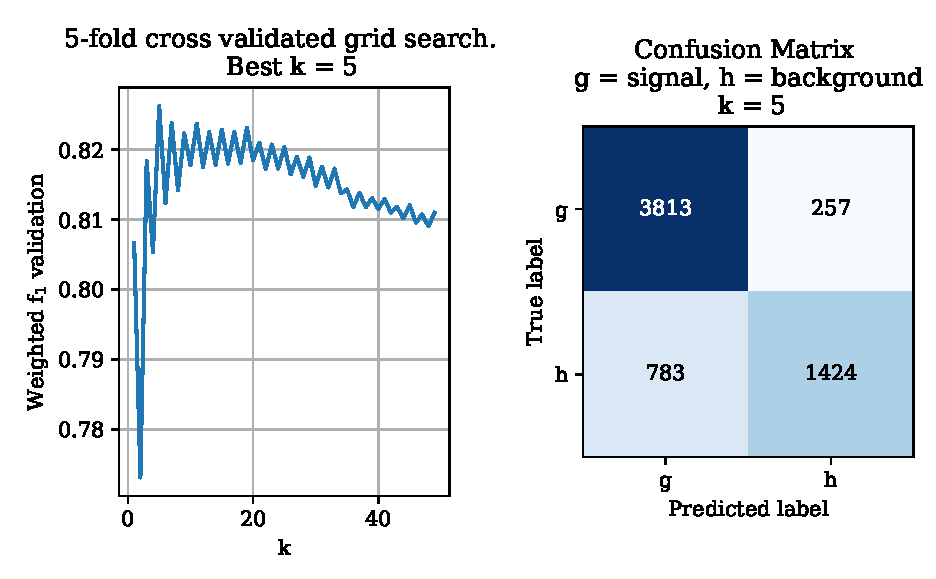
\includegraphics[scale=1]{{figures/kNN_cv_results}.pdf}
\caption{Results from tuned kNN using 5-fold cross validation. The confusion 
matrix was calculated on the test set.}
\label{fig:kNN}
\end{figure*}

\begin{figure}
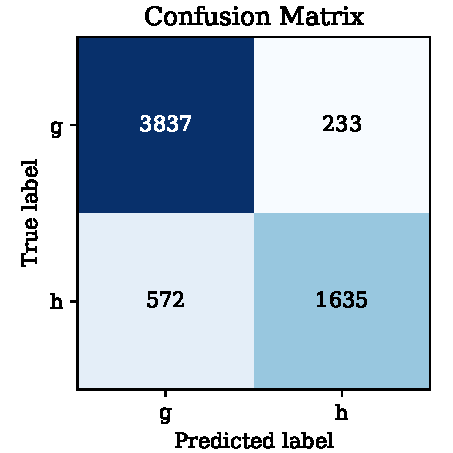
\includegraphics[scale=1]{{figures/nn_confusion_matrix}.pdf}
\caption{Confusion matrix of the MLP model applied to the test set. 
The hyperparameters used can be found in Table \ref{tab:Tune_NN}}
\label{fig:NN_confusion}
\end{figure}

\begin{figure}
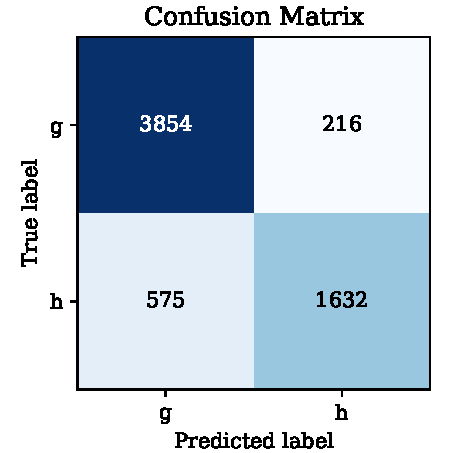
\includegraphics[scale=1]{{figures/xgboost_confusion_matrix}.pdf}
\caption{Confusion matrix of the XGB model applied to the test set.
The hyperparameters used can be found in Table \ref{tab:Tune_XGB}}
\label{fig:XGB_confusion}
\end{figure}



%Figure \ref{fig:Correlation} shows the correlation of the features in the
%training set. Some of the features are highly correlated to each other.

Figure \ref{fig:kNN} shows the result of the cross-validated grid search for the 
optimal $k$ in the kNN model and the corresponding confusion matrix. The value 
of $k$ that resulted in the highest F$_1$ score was $k=5$. The F$_1$ scores for 
the training and test set using this model can be found in Table \ref{tab:F1}.  
We see that the F$_1$ test score is lower than that of the training score, with 
values 0.83 and 0.88 respectively. 

The optimal hyperparameters found using randomised search for the MLP model are 
shown in Table \ref{tab:Tune_NN}. The corresponding confusion matrix and the 
F$_1$ scores are shown in Figure \ref{fig:NN_confusion} and Table \ref{tab:F1} 
respectively. The F$_1$ score for the training and test set are both 0.87. 

The results of the hyperparameter randomised search for the XGB model are shown 
in Table \ref{tab:Tune_XGB}. Figure \ref{fig:XGB_confusion} shows the confusion 
matrix of the XGB model predictions and the F$_1$ scores for the training and 
test sets are shown in Table \ref{tab:F1}. The F$_1$ training score is 0.95, 
which is noticably higher than the test score at 0.88. 

The true positive, true negative, false positive and false negative rates are 
shown in Table \ref{tab:classification_rates} for all three models along with 
the error rates. 

When considering the F$_1$ scores in Table \ref{tab:F1} for the three models , 
the highest test score value was obtained by the XGB model at 0.88, compared to 
0.87 for the MLP and the 0.83. This corresponds to the values seen in the 
confusion matrices of the models in Figure \ref{fig:kNN}, \ref{fig:NN_confusion} 
and \ref{fig:XGB_confusion}. Additionally, the rates of false positives and 
false negatives found in Table \ref{tab:classification_rates} show the lowest 
values for the XGB model, followed closely by the MLP, with the kNN model having 
the highest misclassification rates. 

\begin{table}
\caption{Classification rates for the $k$-nearest neighbour (kNN), multilayer 
perceptron (MLP) and extreme gradient boosting (XGB) models. Hyperparameters used 
can be found in Figure \ref{fig:NN_confusion}, Table 
\ref{tab:Tune_NN} and \ref{tab:Tune_XGB} respectively.}
\label{tab:classification_rates}
  \begin{tabular}{|l|l|l|l|} \hline 
      & \textbf{kNN } \hspace*{2pt}& \textbf{MLP} \hspace*{2pt}& \textbf{XGB} \hspace*{2pt}\\ \hline 
      {True positives}  & 0.607 & 0.611 & 0.613 \\ \hline
      {False negatives} & 0.041 & 0.037 & 0.034 \\ \hline 
      {False positives} & 0.125 & 0.091 & 0.081 \\ \hline 
      {True negatives}  & 0.227 & 0.260 & 0.270 \\ \hline  
      Error             & 0.166 & 0.128 & 0.116 \\ \hline
  \end{tabular}
\end{table}

\section{Discussion}
Although the cross-validation procedure on the kNN model gave the value $k=5$ as 
the optimal amount of neighbours to consider in the algorithm, the F$_1$ score 
in Table \ref{tab:F1} still suggests that there might have been a model overfit. 
The F$_1$ score is lower for the test set, indicating that the predictive 
capability of the model is notably reduced on the test set compared to the 
training set. However, looking at the graph in Figure \ref{fig:kNN} of the 
validation F$_1$ score over $k$, it is clear that it is not possible to improve 
this model any further. This is the downside to using a model that is this simple 
to tune. Generally, the kNN method performs well for being so simple. This implies 
that it could be a good idea to look into more advanced models of this kind. 
Perhaps kernel smoothers or adaptive kNN.

The F$_1$ test and training scores in Table \ref{tab:F1} of the MLP model are 
both 0.87, suggesting that the chosen hyperparameters in Table 
\ref{tab:Tune_NN} did not lead to an overfitted model. Neural networks in 
general are capable of producing highly complex models and are consequently 
prone to overfitting. As this does not seem to have occurred here, it is possible 
we could have been able to find a better-performing model by tweaking the 
hyperparameters further to find more complex models with higher predictive 
power. 

The XGB model F$_1$ test and training scores are 0.88 and 0.95 respectively. 
The large discrepancy in scores is indicative of an overfitted model, and is 
surprisingly the largest difference observed from our three models. Looking at 
the XGB model's hyperparameters in Table \ref{tab:Tune_XGB}, a maximum tree 
depth of 9 might create overly complex models. Additionally, both the optimal 
values for the L1 and L2 shrinkage parameters are small at 0.0074 and 0.0035 
respectively, which might suggest that setting both to zero and choosing to 
instead tune other hyperparameters would yield better results. Some of the 
candidate hyperparameters to tune in an attempt to reduce overfit could be to 
implement the subsample ratios of the features or samples used to grow each 
tree. As the tree would be built on a different data set each iteration, the 
probability of overfitting to certain samples or features would be reduced. 

Despite the discrepancy in F$_1$ training and test scores of the XGB model, the 
model seems to be the best-performing model in our case. Looking at the 
confusion matrices in Figure \ref{fig:kNN}, \ref{fig:NN_confusion}, 
\ref{fig:XGB_confusion}test and Table \ref{tab:classification_rates}, the XGB 
method gave the lowest rate of false negatives, while also 
being the method with the lowest rate of false positives. 

The kNN method is outperformes by both the XGB and MLP models, while the XGB 
model only slightly outperforms the MLP model. As stated previously it may be 
possible to tune the MLP model to perform better. We still argue that the XGB
model is the best model here though, as it is much less computationally expensive.


It is important to keep in mind that this comparison of the model is only for a 
single random train and test split of our data. To get a more statistically 
significant comparison in the future, cross validation should also be used for 
the model selection.

As seen in Figure \ref{fig:Correlation} several features are highly correlated.
If we for instance look at the features \texttt{fConc} and \texttt{fConc1}, 
they are almost $100\%$ correlated to each other and have very similar correlations 
to other features as well. This implies that we could benefit from dimensionality 
reduction here. This could actually improve the kNN model a fair amount as it is 
highly affected by the curse of dimensionality \cite{hastie}.

\section{Conclusion}
We have compared three fundamentally different statistical learning models to 
perform binary classification. XGB seems to be the best performing model for 
our split of the data while also being simpler to tune than the MLP because of 
its reduced computational cost.

In the future it could be benedicial to look into more methods related to kNN, as
it performed well despite being so simple. Performing dimensionality reduction 
could also help kNN perform better.
In addition more time should be spent on tuning the MLP model to see if it can
achieve better performance than XGB. It could also be beneficial to get a 
more statistically stable comparison between the models by using cross validation 
for model selection, avoiding the possibility that our models over or underperform 
on the random train and test split done on the data.

\section*{Acknowledgements}
We want to thank the University of California, Irving for providing us with the
data used in this project.

We are grateful to the developers of the libraries Scikit-learn, XGB, TensorFlow 
and Keras as we used their codes extensively in this project.


%\bibliographystyle{iEEEtran}
\bibliography{bibliography}



\end{document}
